% Name: Hydrogen energy levels
% Description: The energy levels of hydrogen from n = 1 up to ionization, with the first lines of the Lyman and Balmer series as downward transitions.
% Tags: energy levels, hydrogen atom, spectral lines, Bohr model

\usetikzlibrary{arrows.meta}

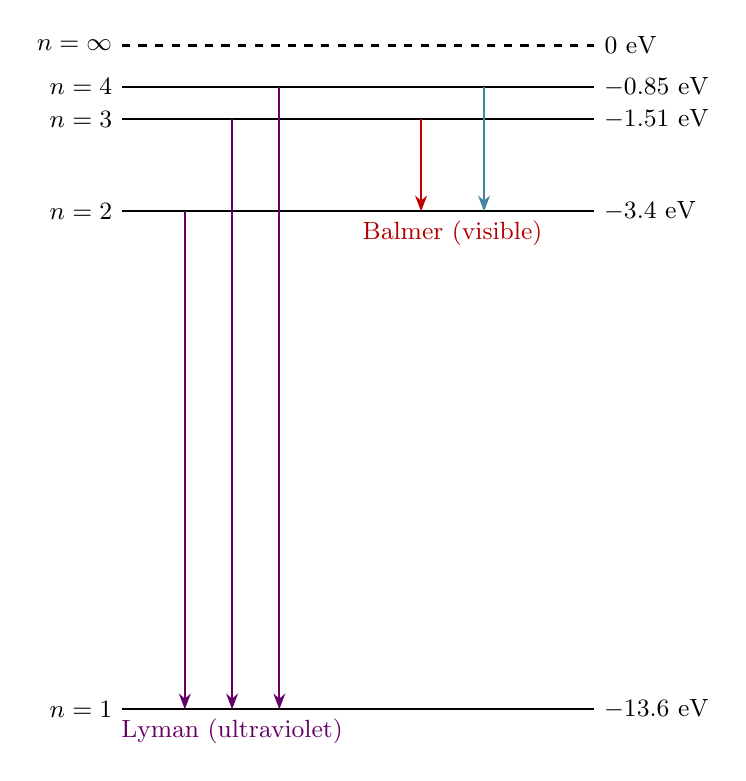
\begin{tikzpicture}[>={Stealth[length=2mm]}, y=0.62cm, every node/.style={font=\small}]
  % E_n = -13.6 / n^2 eV, drawn to scale.
  \foreach \n/\e in {1/-13.6, 2/-3.4, 3/-1.51, 4/-0.85} {
    \draw[thick] (0,\e) -- (6,\e);
    \node[left] at (0,\e) {$n = \n$};
    \node[right] at (6,\e) {$\e$ eV};
  }
  \draw[thick, dashed] (0,0) -- (6,0) node[right] {$0$ eV};
  \node[left] at (0,0) {$n = \infty$};
  \foreach \from/\x in {-3.4/0.8, -1.51/1.4, -0.85/2}
    \draw[->, thick, violet!80!black] (\x,\from) -- (\x,-13.6);
  \node[violet!80!black, below] at (1.4,-13.6) {Lyman (ultraviolet)};
  \foreach \from/\x/\c in {-1.51/3.8/red!75!black, -0.85/4.6/cyan!60!black}
    \draw[->, thick, \c] (\x,\from) -- (\x,-3.4);
  \node[red!70!black, below] at (4.2,-3.4) {Balmer (visible)};
\end{tikzpicture}
